\chapter{MWL}
\label{chapter:MWL}
In diesem Kapitel werden neben der MAGIC Lichtkurve noch Lichtkurven anderer Experimente in anderen Wellenlängen dargestellt, die im Rahmen einer Multiwellenlängen -Kampagne (MWL-Kampagne)  genommen wurden und mit den MAGIC Daten verglichen.
Es stehen dazu Daten im Energiebereich zwischen Radiowellen und Very High Energy Gamma Rays zur Verfügung.
Die MWL-Kampagne fand zwischen dem 23.12.2011 und dem 01.06.2012 statt und war die Fortsetzung einer früheren MWL-Kampagne von 2009.
Genauso wie während der Vorgängerkampagne befindet sich innerhalb der Beobachtungszeit kein Flare.
Das Ziel dieser Kampagne ist, den Fluss und die spektrale Entwicklung der Breitband-Emission über eine lange Zeitspanne zu untersuchen, wobei jeweils tageweise Daten genommen wurden.
Während es viele Untersuchungen zu den Emissionsszenarien bei Flares gibt [siehe z.B. \cite{Mrk421Flare}], wurde der ruhige Zustand von Mrk 421 abgesehen von \cite{MWL2009} nicht sehr ausführlich untersucht.
Mit Hilfe von diesen Daten, können grundlegende Emissionsprozesse untersucht werden.

Blazare wie Mrk 421 sind in allen Wellenlängen sehr variabel.
Die Spektrale Energieverteilung (SED) wird von der Jet-Emission dominiert und besitzt eine zweihöckrige Struktur.
Der erste Höcker findet sich bei niedrigen Energien [Radio, optisch, Röntgenstrahlen] und der andere bei höheren Energien [Röntgen, Gamma, VHE].
Während der Ursprung des niederenergetischen Höckers Synchrotron-Emission von relativistischen Elektronen ist, ist der Ursprung des hochenergetischen Höckers noch nicht genau bekannt.
Sowohl leptonische als auch hadronische Modelle versuchen die Struktur zu erklären.
Um Modelle für den hochenergetischen Höcker zu machen, sind weiterhin Beobachtungen in verschiedenen Wellenlängen nötig. 
 

\section{Teilnehmer an der MWL-Kampagne}
Von den folgenden Experimenten, die sich an dieser Kampagne beteiligt haben, stehen mir Daten zur Verfügung:

\begin{itemize}
 \item MAGIC: eigene Analyse
 \item \textit{Swift}/XRT: \textit{Swift} ist ein Satellitenexperiment mit dem Ziel GRBs zu detektieren und zu untersuchen.
  Dabei liegt die Priorität darauf, den Ursprung von GRBs zu finden, die Entwicklung der GRBs und die Wechselwirkung mit der Umgebung zu untersuchen und die GRBs zu klassifizieren.
  Dazu sind drei Instrumente an Bord, die in verschiedenen Wellenlängen sensitiv sind. 
  Mit \textit{Swift} können Gammastrahlen, Röntgenstrahlen, UV-Strahlung und optisches Licht detektiert werden.
  Mit Hilfe des Burst Alert Telescope (BAT) werden Teilchen mit Energien zwischen $\SI{15}{keV}$ und $\SI{150}{keV}$ untersucht.
  Das UV/Optical Telescope (UVOT) detektiert im sichtbaren und im UV-Bereich (170-$\SI{600}{nm}$).
  Die für diese Analyse vorliegenden Daten sind Daten des Xray Telescop (XRT), womit Röntgenstrahlung mit einer Energie zwischen $\SI{0,3}{keV}$ und $\SI{10}{keV}$ detektiert wird.\cite{Swift}
 \item OVRO: Das Owens Valley Radio Observatory (OVRO) befindet sich in der Nähe von Bishop in Kalifornien im Osten der Sierra Nevada.
  Es ist ein Radioteleskop mit einem Durchmesser von $\SI{40}{m}$, welches bei $\SI{15}{GHz}$ operiert.
  Ziel dieses Experimentes ist das Monitoring von ca. 1200 Blazaren.
  Dabei wird jede Quelle in einem Abstand von 2 Tagen regelmäßig beobachtet.
  Diese Daten werden dann mit den Daten, die mit \textit{Fermi} von den gleichen Quellen aufgenommen wurden, verglichen und Korrelationen in der Variabilität gesucht.
  Letztendlich ist ein genaueres Verständnis von Emissionsprozessen in AGNs das Ziel.\cite{OVRO}
 \item Metsahovi: Metsahovi ist ein Radioteleskop mit einem Spiegeldurchmesser von $\SI{14}{m}$. 
  Es befindet sich in Finnland, in Kirkkonummi, und beobachtet Frequenzen zwischen $\SI{2}{GHz}$ und $\SI{150}{GHz}$.
  Mit dem Teleskop werden hauptsächlich extragalaktische Quellen beobachtet, aber auch die Sonne und es nimmt an VLBI (Very Large Baseline Interferometry)-Beobachtungen teil.\cite{Metsahovi}
 \item Optische Teleskope: Für diese Analyse stehen die Daten einiger optischer Teleskope zur Verfügung, deren Datennahme unter Einsatz des R-Filters geschah.
  Im Folgenden werden diese Teleskope aufgelistet:
 \begin{itemize}
  \item Crimean: Das Crimean Astrophysical Observatory befindet sich in Nauchny auf der Krim, Ukraine, und beherbergt verschiedene optische Teleskope.\cite{Crimean}
  \item KVA: Das Kungliga Vetenskaplika Academy (KVA)-Teleskop befindet sich genauso wie die MAGIC Teleskope auf dem Roque de los Muchachos auf La Palma.
    Es handelt sich um ein Teleskop mit einem Spiegeldurchmesser von $\SI{35}{cm}$.
    Die Daten sind alle im Johnson R-Band genommen und weiterverarbeitet.\cite{KVA}
  \item Perkins: Das Perkins Telescope ist ein $\SI{72}{inch}$ ($\SI{1,83}{m}$)-Teleskop, das zum Lowell Observatory in Arizona, USA, gehört.
    Mit diesem Teleskop werden vor allem Wide-Field-Bilder aufgenommen und es dient der Multi-Objekt-Spektroskopie.
    Unter anderem soll mit diesem Teleskop auch die variable Natur von Blazaren untersucht werden.\cite{Perkins}
  \item ROVOR: Das Remote Observatory for Variable Object Research (ROVOR) gehört zur Brigham Young University.
    Es handelt sich um ein optisches Teleskop mit einem Spiegeldurchmesser von $\SI{16}{inch}$ ($\SI{0,41}{m}$) und es befindet sich $\SI{12}{km}$ nordwestlich von Delta (Utah).
    Es wurde gebaut um variable Objekte wie AGNs dauerhaft zu monitoren, um die existierenden Modelle für AGNs zu verbessern.
    ROVOR nimmt am Gamma Ray Burst Coordinate Network (GCN) teil und beobachtet die Afterglows im optischen Wellenlängenbereich.\cite{ROVOR}
  \item St. Petersburg: Das Pulkovo Astronomical Observatory befindet sich südlich von St. Petersburg auf einer Höhe von $\SI{75}{m}$ über NN.\cite{StPetersburg}
  \item TeB: Das Bradford Robotic Telescope ist Teil des Observatorio del Teide auf Teneriffa, Kanarische Inseln. 
    Es befindet sich auf einer Höhe von $\SI{2400}{m}$ und wird robotisch betrieben.\cite{TeB}
  \item NMSkies: New Mexico Skies bietet einen Standort und Support für dort aufgestellte Remote Teleskope. 
    Das Teleskop NMSkies GRAS-001 befindet sich in Mayhill, New Mexico, USA.\cite{NMSkies}
 \end{itemize}

 \item \textit{Fermi}: Das Large Area Telescope (LAT) befindet sich an Bord des \textit{Fermi} Gamma-Ray Space Telescope und detektiert sowohl Gamma-Strahlen als auch geladene kosmische Strahlen.
  Das Teleskop beinhaltet einen Antikoinzidenzdetektor, durch den das Photon im Gegensatz zur geladenen kosmischen Strahlung wechselwirkungsfrei fliegt. 
  Danach wechselwirkt es mit Atomen in einer der Schichten aus Wolfram-Folie und produziert ein Elektron-Positron-Paar, welches getrackt wird.
  Die finale Energie dieses Elektron-Positron-Paars wird dann in einem Kalorimeter gemessen.
  Das Entdecken und Überwachen von variablen Quellen und GRBs sowie die Erstellung von aktuellen Katalogen von hochenergetischen Quellen gehören zu den Hauptzielen von \textit{Fermi}.\cite{Fermi} 
\end{itemize}

\section{Lichtkurven}
In Abb.\ref{LC_MWL} befinden sich die Lichtkurven der verschiedenen Experimente, die im Zeitraum zwischen dem 23.12.11 (MJD: 55918) und dem 01.06.12 (MJD: 56079) gemessen wurden.

\begin{sidewaysfigure}
%\begin{sidewaysfigure}
%\begin{figure}
    \centering
    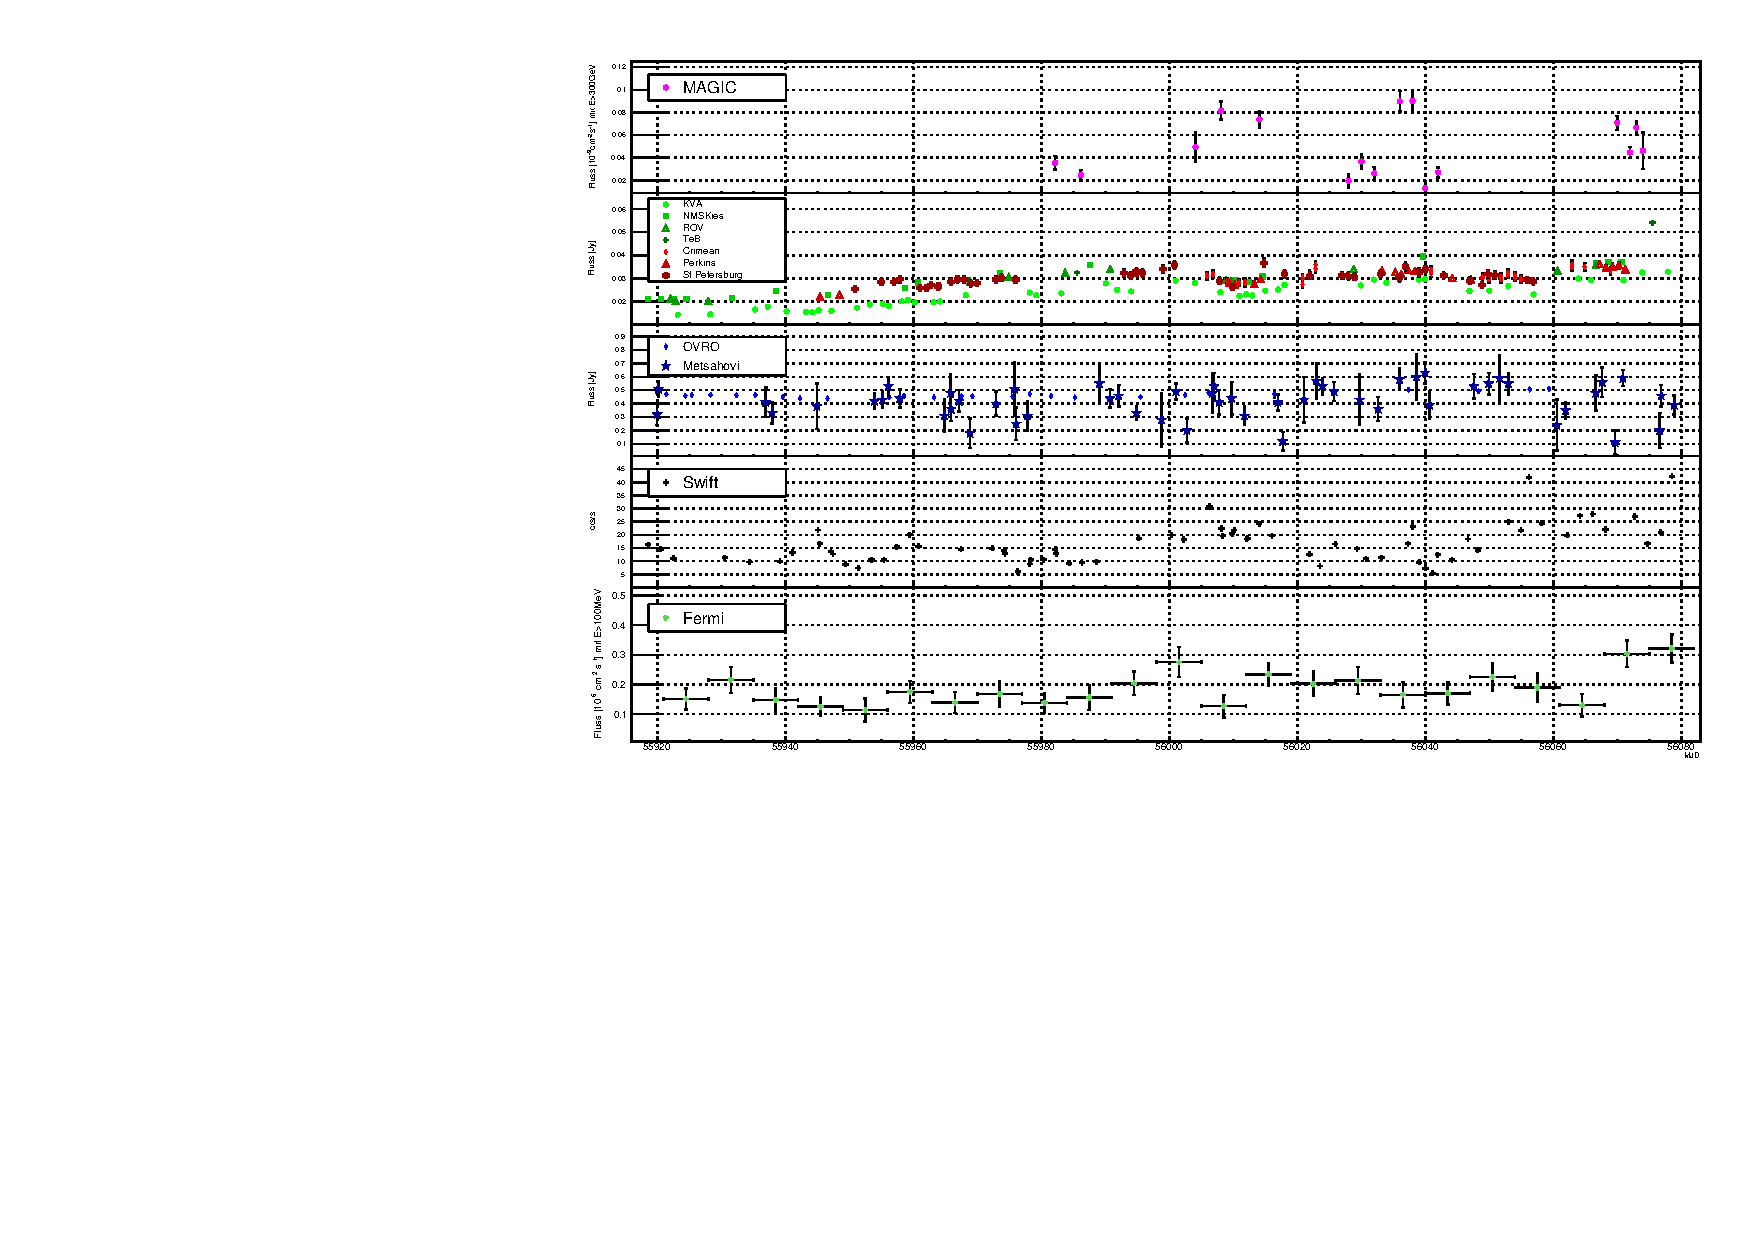
\includegraphics[width=1\linewidth]{./Plots/05_MWL/LC_final.pdf}
    \caption{Alle Lichtkurven, die während der MWL-Kampagne aufgenommen wurden: von oben nach unten: VHE, Optische Teleskope, Radio, Röntgen, Gamma}
    \label{LC_MWL}
%\end{figure}
\end{sidewaysfigure}

Leider hat MAGIC an nur 16 Tagen davon Daten genommen, weswegen die Lichtkurve im Vergleich zu den anderen Experimenten recht kurz ist, bzw. große Lücken aufweist.
Auf den ersten Blick weist die Lichtkurve eine variable Struktur auf, was in \autoref{sec:Variabilitätsuntersuchung} noch getestet wird.

Die optischen Lichtkurven der verschiedenen Teleskope liegen insgesamt auf einem ähnlichen Niveau, wobei KVA immer etwas niedriger ist.
Die meisten Daten stammen von KVA (Beobachtung an 48 Tagen), dem St. Petersburger Teleskop (Beobachtung an 46 Tagen) und dem Crimean Astrophysical Observatory (Beobachtung an 35 Tagen).
Die Variabilität im Fluss zwischen den verschiedenen Teleskopen ist ähnlich. 
Einige Schwankungen sind zu erkennen und zum Ende der Lichtkurve nimmt das Niveau etwas zu.

Im Radiobereich sind bei den OVRO-Daten kaum Variabilitäten zu erkennen. 
Die Daten von Metsahovi unterliegen größeren Schwankungen, sind aber auch mit einem größeren Fehler behaftet.
Quantativ wird dieses Verhalten in \autoref{sec:Variabilitätsuntersuchung} gezeigt.

Die Daten des Röntgenteleskops \textit{Swift}, welches eine sehr konstante Datennahme aufweist, zeigen einen eher variablen Fluss, was im Folgenden noch überprüft wird.

Die Daten von \textit{Fermi}-LAT sind gemittelte Resultate von einer Woche, zeigen also keine täglichen Schwankungen.
Aufgrund des Mittelns und der dadurch Nicht-Vergleichbarkeit mit den anderen Experimenten wird im Folgenden keine Variabilität berechnet.

Insgesamt kann man erkennen, dass die Variabilität in der VHE-Lichtkurve auf Zeitskalen von ca. einem Tage auftritt, während der Fluss im optischen oder Röntgenbereich eher innerhalb einer Woche ansteigt und wieder abnimmt. 
Die Radiolichtkurven weisen keine sichtbaren Variabilitäten auf.

\section{Variabilitätsuntersuchung}
\label{sec:Variabilitätsuntersuchung}
Obwohl es in der Zeit der MWL-Kampagne zu keinem Flare kam, sind die Daten von Mrk421 variabel.
Um quantifizieren zu können, wie variabel die Daten sind, wird für jeden Energiebereich die Fractional Variability nach \cite{Vaughan} ausgerechnet.
Der Wert für die Fractional Variability $F_{var}$ wird mit $S$: der Standardabweichung der N Flussmessungen, $\langle \sigma_{err} \rangle$: dem mittleren quadrierten Fehler und $\langle x \rangle^2$: dem Quadrat des mittleren Photonflusses berechnet:

\begin{equation}
 F_{var}=\sqrt{\frac{S^2-\langle \sigma_{err} \rangle^2}{\langle x \rangle^2}}.
\end{equation}

Der Fehler davon ist \cite{FehlerVariability} entnommen: 

\begin{equation}
 \Delta F_{var}=\sqrt{F_{var}^2+err(\sigma_{NXS}^2)}-F_{var}
\end{equation}

mit $err(\sigma_{NXS}^2)$ aus \cite{Vaughan}:

\begin{equation}
 err(\sigma_{NXS}^2)=\sqrt{\left(\sqrt{\frac{2}{N} \frac{\langle \sigma_{err}^2 \rangle}{\langle x \rangle^2}} \right)^2 + \left( \sqrt{\frac{\langle\sigma_{err}^2 \rangle}{N} \frac{2F_{var}}{\langle x \rangle}} \right)^2}.
\end{equation}

Damit die Berechnung von $F_{var}$ stabil ist, wird eine Mindestanzahl von 20 gemessenen Datenpunkten empfohlen.
Obwohl die MAGIC-Daten nur aus 16 gemessenen Punkten besteht, wird trotzdem zum Vergleich einmal die Variabilität ausgerechnet.
Die berechneten Werte für die Variabilität $F_{var}$ mit Fehler $\Delta F_{var}$ sowie die Anzahl der Messpunkte $N$ befindet sich in \autoref{tab:Variabilitäten}, bzw. in \autoref{LC_Variabilities}.


\begin{table}[!h]
\centering
\caption{Anzahl der Messpunkte, sowie die berechneten Variabilitäten für die verschiedenen Lichtkurven.}
\label{tab:Variabilitäten}
\begin{tabular}{llccc}
  \toprule
  Wellenlänge & Experiment & N & $F_{var}$ & $\Delta F_{var}$\\
  \midrule
  \midrule
  Radio & Metsahovi & 55 & 0,1390 & 0,0319 \\
  &OVRO & 27 & 0,0381 & 0,0036 \\
  optisch &KVA & 48 & 0,2227 & 0,0031 \\
  &St. Petersburg & 46 & 0,0768 & 0,0067 \\
  &Crimean & 35 & 0,0586 & 0,0075 \\
  Röntgen & \textit{Swift} & 70 & 0,4428 & 0,0015\\
  Gamma & MAGIC & 16 & 0,4913 & 0,0380 \\
  \bottomrule
\end{tabular}
\end{table}


\begin{figure}
    \centering
    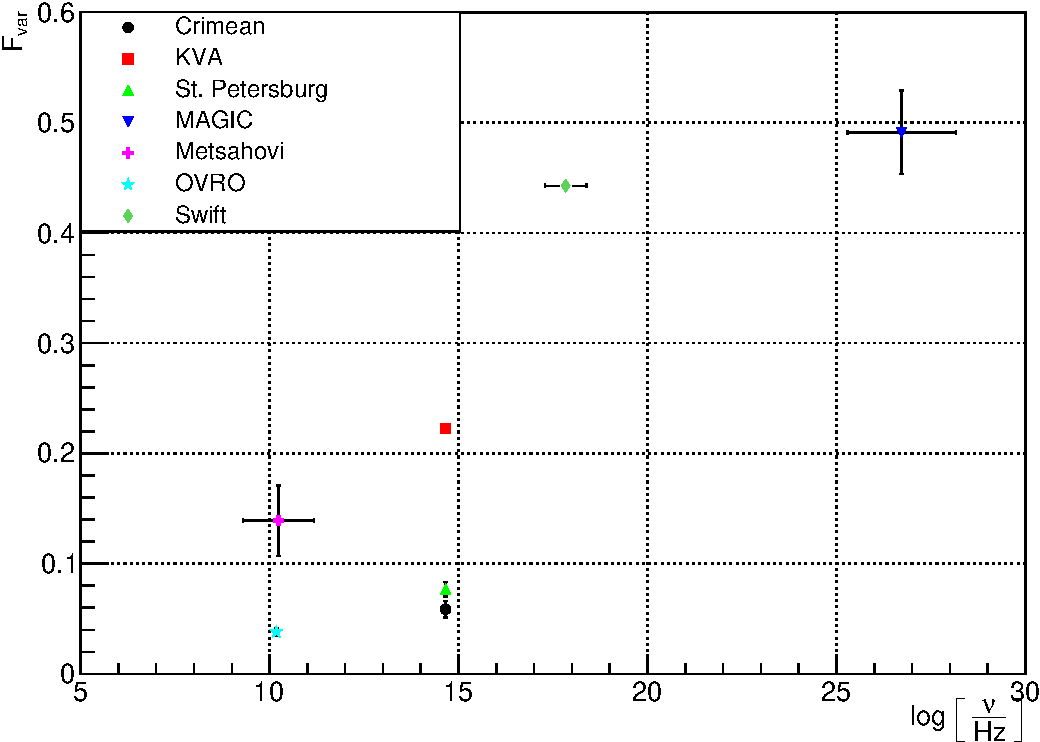
\includegraphics[width=0.8\textwidth]{./Plots/05_MWL/PlotVariabilities.pdf}
    \caption{Variabilitäten für verschiedene Wellenlängen.}
    \label{LC_Variabilities}
\end{figure}

\autoref{LC_Variabilities} zeigt die Variabilitäten in den einzelnen Wellenlängen, wobei die Breite des x-Balkens den Energiebereich angibt, in dem die jeweiligen Instrumente messen.
\autoref{LC_Variabilities} zeigt, dass die Variabilität von Mrk421 im Radio- und im optischen Bereich sehr niedrig ist, während die AGN im Röntgen- und im Gamma-Bereich Variabilität aufweist, wobei beachtet werden muss, dass der Wert für MAGIC mit Vorsicht betrachtet werden muss, da die Anzahl der Datenpunkte niedrig ist.
Insgesamt lässt sich sagen, dass die Variabilitäten mit steigender Frequenz ebenfalls ansteigen.
Die hier berechneten Variabilitäten sind ähnlich zu den berechneten Werten für Mrk421 von 2009 \cite{MWL2009}.
